\section{Introduction}

\begin{figure*}[t]
\centering
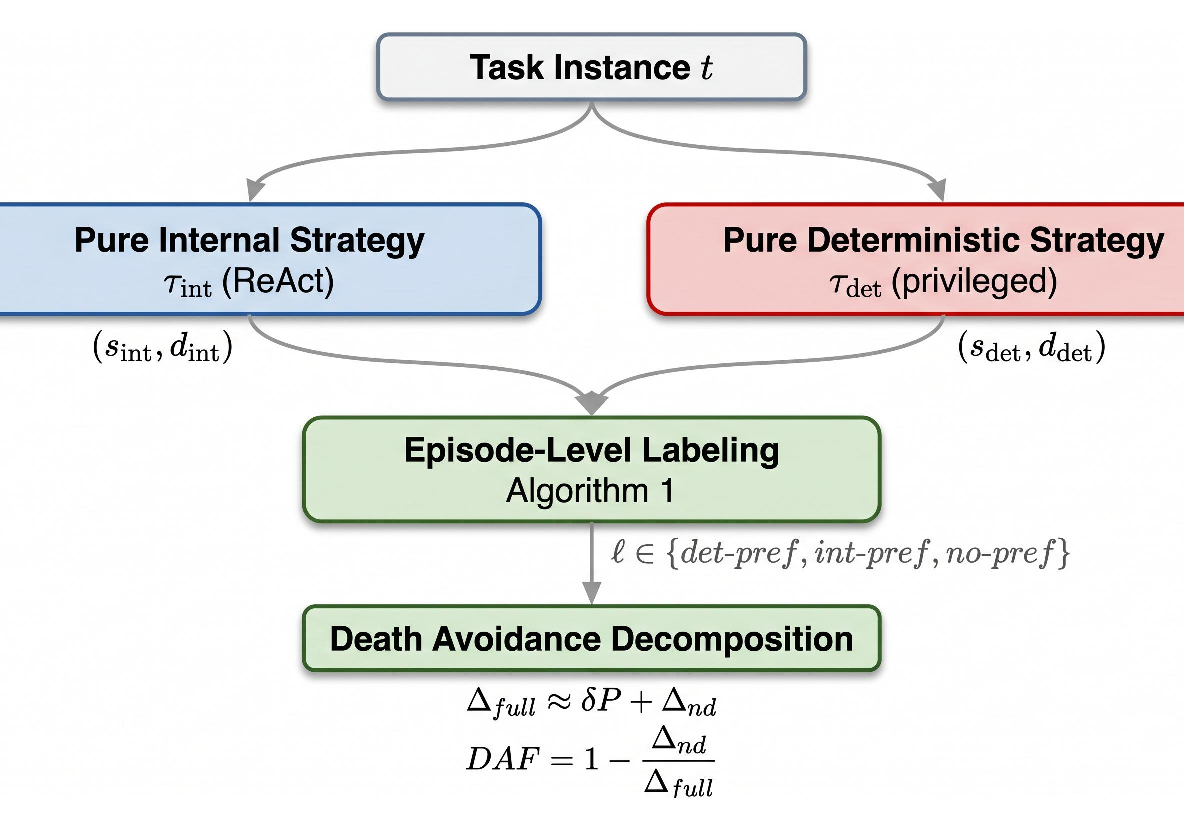
\includegraphics[width=0.95\textwidth]{figures/pipeline_overview.pdf}
\caption{Counterfactual episode collection and analysis pipeline. Each task instance is run under both pure strategies independently, producing episode-level labels via Algorithm~\ref{alg:labeling}.}
\label{fig:pipeline}
\end{figure*}

Large language models deployed as interactive agents must repeatedly decide \emph{how} to compute: reason internally, or delegate to an external tool.
Existing routing methods, whether inserting API calls by perplexity reduction~\citep{toolformer-2023}, decomposing tasks into tool-augmented programs~\citep{art-2023,chameleon-2023}, or adaptively selecting reasoning depths~\citep{cogrouter-2026,ares-2026} and model tiers~\citep{mtrouter-2026,budget-aware-routing-2026}, share an implicit assumption: that routing signal stems from diverse sources and a learned router can exploit it. But before training a router, we should understand what mechanistic signal drives the routing preference. If signal collapses to a single dominant mechanism, a learned step-level router may not be the right solution.

We propose an \emph{episode-level counterfactual diagnostic framework} to address this prior question. The framework compares pure-strategy outcomes (internal-only vs.\ deterministic-only) and introduces the Death Avoidance Factor (DAF) to decompose the routing score gap into death-avoidance and non-death components (\S\ref{sec:collection}--\ref{sec:daf}). Operating at episode granularity is essential: per-step oracle labeling degenerates under sparse terminal rewards (97.4\% tie rate in ScienceWorld; \S\ref{sec:collection}).

Applied to ScienceWorld~\citep{scienceworld-2022}, the framework reveals that \textbf{78.9\% of non-tie routing labels arise from death asymmetry}, where the internal strategy triggers a catastrophic failure while the deterministic strategy survives. This pattern replicates across three architecturally distinct model families (7--70B parameters) and intensifies at larger scale, where death avoidance accounts for the entire performance gap (\S\ref{sec:cross-model}--\ref{sec:agent-improvement}). Always-deterministic matches 96.3\% of oracle routing decisions; a trained step-level router fails to exceed this trivial baseline (\S\ref{sec:baselines}--\ref{sec:router-diagnostic}). Boundary probes on MATH and ALFWorld show that the framework distinguishes qualitatively different mechanisms, including environments with no routing signal and those driven by information asymmetry (\S\ref{sec:cross-env}).

Our contributions: (1)~An \textbf{episode-level counterfactual diagnostic framework} and the DAF metric that decompose routing signal into mechanistic components before any router is built, overcoming per-step oracle degeneracy in sparse-reward environments.
(2)~Evidence that \textbf{routing signal in ScienceWorld is death-dominated}: 78.9\% of non-tie labels trace to death asymmetry, replicated across three model families and two scales (7B and 70B). A ${\sim}$50-episode pilot suffices for practitioners to assess whether learned routing adds value (Appendix~\ref{app:decision-framework}).
(3)~\textbf{Boundary probes} on MATH and ALFWorld showing the framework can diagnose qualitatively different routing mechanisms, while clarifying that full quantitative validation remains specific to ScienceWorld.
